\documentclass[11pt]{article}
\usepackage[tbtags]{amsmath}
\usepackage{amsfonts}
\usepackage{amssymb}
\usepackage{graphicx}
\usepackage{hyperref}
\usepackage{enumerate}


%%Math packages
\usepackage{amssymb,amsmath}


\usepackage{epsfig}
\usepackage{calc}
\usepackage{color}

%\renewcommand{\baselinestretch}{1.2}
%\setlength{\topmargin}{-0.5in}
%\setlength{\textwidth}{6.5in}
%\setlength{\oddsidemargin}{0.0in}
%\setlength{\textheight}{9.1in}

%\newlength{\pagewidth}
%\setlength{\pagewidth}{6.5in}
%\pagestyle{empty}
%\setlength{\topmargin}{0.0in}
%\setlength{\columnsep}{2.0pc}
%\setlength{\footheight}{0.0in}
%\setlength{\headheight}{0.0in}
%\setlength{\headsep}{0.0in}
%\setlength{\oddsidemargin}{0.0in}
%\setlength{\parindent}{1pc}
%\textheight 8.75in
%\textwidth 6.8in
\def\pp{\par\noindent}
\DeclareGraphicsExtensions{.pdf,.png,.jpg}



\begin{document}

\title{\textbf{Linux - System Call Inherit}}
\author{Group 12 \\ Prankur Gupta\hspace{1.9cm} Sumit Bagga\hspace{1.9cm}Abhishek shukla\\
108492684 \hspace{2.5cm}108235636 \hspace{2.5cm}107598884\\ \{prgupta, ssbagga, ashuklaravis\}@cs.stonybrook.edu}
\date{April 29,2012}
\maketitle

\section{Abstract}
\medskip
System calls provide the interface between a process and the operating
 system (kernel). We as a user process, can request kernel to perform some
previleged tasks, by calling these system calls. When a user process invokes
a system call, the CPU switches to Kernel Mode and starts the execution of
kernel function. There is a set of such system calls defined in Linux, represented
by a unique system call number. For each of these system call, there is a unique
system call handler. Any changes in the system call or their handler, must be followed
by recompiling the kernel so that  the changes can take affect. So, it is neither easy to
change or add a system call as per users need, nor does Linux provides some
implementation for doing that.Adding a new system call to the kernel and then 
creating programs that use this call take away the program's portability.
Adding a system call can also introduce a serious security problem into your system. 
The best solution is to write our own system calls but adding them statically or even as a module
requires changes in the kernel code which may cause inconsistency and takes away kernel portability.
Unlike Linux, BSD provides facilities to override the default system call vector. We aim to 
provide user an additional functionality to override the system call vector and also its
subsequent child processes will also use that overridden vector only. For this we created
a module to register and deregister the vector names, which have the overridden system call
number and their function implementation. The user can choose to use the overridden system call vector through ioctl, which populates the private data field of $task\_struct$ of that process with the address of the list of system call and their function
implementation. 

\section{Introduction}


In Linux, accessing the $sys\_call\_table$ by user process or even
LKM (Lodable Kernel Module) is not possible. And in order to add a new system call we need to add an entry
in the $syscall.h$.  But there can be a need of adding new functionality in form of system calls. So,
we need an implementation for providing that functionality. We came accross many ideas for implementing
this e.g. 
\begin{enumerate}[(a)]
\item
creating a new system call for this purpose, 
\item
intercepting system calls in user level library, 
\item
overriding the global system call table. 
\end{enumerate}
Among these three, we decided to go with the last one, as it
seemed reasonably better in accordance to what we aim to achieve. It is sometimes required that an application wants its processes to use a set of system calls only and might want their own implementation of those system calls, e.g. An application while calling 
exec() might want to log this information in a file, so we can wrap their exec() syscall to do this task.

Now, if we want to override the global system call table then we need to identify which process needs
what additional functionality. We can't just create another syscall table and ask our process to use that
if they needed additional functionality. We needed a way to generalise it. So, we decided to create 
new overridden system call tables on per process basis. As this provides user specific functionalities.

We are maintaining a per-process system call vectors information in the private field of their
$task\_struct$. The process needs to choose the system call vector beforehand i.e. before calling any system
call, through ioctl of the "$ioctl\_device$" character device loaded also via module. The list of all the possible
overridden system call vectors can be available in "/proc/" filesystem. The reason for choosing "/proc/" filesystem 
is because its easy to understand and handling kernel internal data structures inside it is also easy. 
A user process can override the default $sys\_call\_table$ with any of these registered system call vectors.
Once a user process $task\_struct$ is populated by the address of the $syscall\_vector's$ address,
whenever this process calls a system call, we access the overridden or wrapped functionality as desired by user. 
Now when a process is forked or cloned, the $task\_struct$ is copied to its child, so the child will perform
as a shadow of its parent whenever it calls the overridden system call vectors.

\section{Background}

Each system call has a unique number by which it is represented and a unique handler (internal kernel data structure).
This unique number is what is stored in the $eax$ register before control is given to kernel code. Each system call
has to follow two fixed intructions i.e. sysenter and sysexit. They represents the entry and exit of the kernel control
of the system call. Whenever a user process requests for privileged access through system call, an interrupt is
generated \textbf{int 0x80}. After this interrupt, context switch happens and all the interrupts are disabled.
The interrupt calls the respective system call defination through $sys\_call\_table$ based on the value of the $eax$
register. When the desired work is done, the control passes  to user space after executing sysexit and the
interrupts are enabled again.

\section{Motivation}

System Call Inheritance can prove to be a powerful scheme and can have the following applications: 

\medskip
\noindent
\textbf{a)} System calls can be modified to suit application specific usage of the OS. For Ex Logging, Profiling etc 

\noindent
\textbf{b)} Security Applications: Depending on the security level of the user, the set of system calls allowed can be different. 

\noindent
\textbf{c)} Additional functionality can be added to the existing system calls fairly easily, maintaining the portability of the kernel. Kernel capable of allowing a user to extend system calls without changing the behaviour of other applications on the system is required. 

\noindent
\textbf{d)} BSD has the feature of overriding system call table at a process level thus allowing access to kernel data structures without having a risk of writing an unsecure or bug prone kernel code. 

\noindent
\textbf{e)} By this approach a user can extend system calls without changing behaviour of other applications on system.

\medskip
\noindent
This can provide portability of kernel and ease of performing desired priviledge work, without modifying a lot of kernel code.

\section{Major Features}

\begin{enumerate}[(a)]

\item
System call overriding: User defined functions are overridden when normal system calls are made. This paper discusses one of the possible ways to bring this functionality into the linux kernel. 

\item
System call wrapping: Even though it easy to implement system call wrapping once system call overriding is implemented, it proves to be important; a feature that could be used for loggin purposes. 

\item
System call inheritance: The system call vector which is used to override the system calls in the parent will be inherited into the child process.
 
\item
Ioctl: We have used ioctl to add the overriding system call vector to the processes task structure. We chose to use ioctl and not a modified version of exec as we can add/remove/change the system call vectors at runtime. 

\item
Helper functions: We have added all the required helper functions to register, unregister system call vectors etc. 

\end{enumerate}

\section{Design}

In this section we are discussing about our approach to acheive our desired aim. We have designed two $primary$ modules and 
two $helper$ modules for testing

\medskip
\noindent
\textbf{a)} Module to register and unregister the system call vector

\noindent
\textbf{b)} Module for a character device through which we would be sending ioctl's.


\noindent
\textbf{c)}  Two modules as an implementation of new system call vectors having overridden or wrapped syscall functions.


\medskip
\noindent
In the first module and most important \textbf{reg\_unreg.ko}, we are regitering/deregistering the system call vector. These vectors are visible to the user in the
\textbf{proc} filesystem in the file named as \textbf{syscall\_vectors}. We create a file in $proc$ filesystem using 
$create\_proc\_entry()$ function and defines $pde \rightarrow read\_proc$ by our own implemented function i.e.$show\_vectors$.

\medskip
\noindent
Proc filesystem is used because we do not require users to write in the file, or do any other file operations. 
Further proc filesystem allows an easy hook to data structures defined in kernel. Also provides easy way to access them using
 callback functions available like $read\_proc$ and $write\_proc$.
 Here, $write\_proc$ is not implemented since we don't want user to write anything to our data structures.
This module contains four exported functions:

\begin{center}
	 int register\_syscall(char *vector\_name, unsigned long vector\_address); \hfill(1)\\
	int unregister\_syscall(char *vector\_name, unsigned long vector\_address);\hfill(2)\\
	unsigned long get\_vector\_address(char *vector\_name);\hfill(3)\\ 
	int reduce\_ref\_count(char *vector\_name);\hfill(4)
\end{center}

As the name suggests, they are used for registering, deregistering ,showing the registered vectors and reducing the refererence count of the vectors used which are defined in $syscall\_vectors$ file in $proc$ filesystem. We are using $mutex$ on $list\_lock$ to protect accesses of registering / deregistering / showing / reducing reference count of the vector.  We are using the following structure of vector :

\medskip
\noindent
struct new\_vector \{   

\hspace{2.9cm}char vector\_name[MAX\_VECTOR\_NAME\_LEN];

\hspace{2.9cm}unsigned long vector\_address;

\hspace{2.9cm}int ref\_count;

\hspace{2.9cm}struct module *vector\_module;

\hspace{2.9cm}struct new\_vector *next;

\hspace{2.6cm}\};

\medskip
\noindent
where, 

struct module * stores the information of the registering module

vector\_address contains the address of the syscall\_vector structure

\medskip
\noindent
struct syscall\_vector \{  

\hspace{3.2cm}struct overridden\_syscall sys\_call;

\hspace{3.2cm}struct syscall\_vector *next;	

\hspace{3.0cm}\};

\bigskip
\noindent
struct overridden\_syscall \{

\hspace{3.7cm}int syscall\_no;

\hspace{3.7cm}unsigned long function\_ptr;

\hspace{3.5cm}\};


\medskip
\noindent
The second module \textbf{proc\_test.ko} is for registering the character device $\textbf{ioctl\_device}$ with Device number 121.
This device is used for sending two ioctl's namely IOCTL\_SET\_VECTOR and IOCTL\_REMOVE. 

\medskip
IOCTL\_SET\_VECTOR when called, increases the reference count of this module and retrieves the vector\_address
of the desired vector name through externed method (3) which in turn increases the reference count of that vector and adds that address into the new \textbf{void *} field created  inside the \textbf{task\_struct} of the calling process. The added field in the task\_struct is void *syscall\_inherit\_data.

IOCTL\_REMOVE when called, removes the particular vector name from the task\_struct of the calling processm and also 
 reduces the reference count of the vector name and also calls $module\_put()$, thus decreasing the reference count of the
module itself.

\medskip
\noindent
All these functions of adding/ removing the vector address in the task\_struct of the calling process are safeguarded by
a $mutex$ lock.

\medskip
\noindent
The module $\textbf{link\_vector.ko}$ and $file\_ops\_vector$, create a system call vector i.e. $syscall\_vecter$ structure using a set of  system call numbers and their function implementation address, which we want to override. It then registers
the vector by calling the exported function (1). Similarly, it can unregister the vector, by calling (2).

Apart from this, we have created a call to our defined function inside system call entry code in $entry\_32.S$, which checks
whether the $void $* field of task struct is NULL or not. 


\section{Implementation}

We now give the implementation details of our design.
We used Linux 3.2.2+ kernel for our implementation. For every system call , the
kernel jumps to the appropriate handler in the $sys\_call\_table$, based on the system call number.
The system call number is stored in the $eax$ register. The system call table is in the form of
linked list. We search for system call handler corresponding to the number. The
parameters to the system call are passed in the kernel stack and we define handler as $asmlinkage$ function which informs compiler to take arguements from the stack. After return from the handler, the return
value is stored in the $\%eax$ register.

We check the $void$ * fieldof the $task\_struct$ of the process, whether it is $NULL$ or contains
the address to the $syscall\_vector$. If it is $NULL$, I'm passing the control as it is,
$\%eax$ register containing a fixed return value, which is then replaced by the value of original $\%eax$ registered popped from the kernel stack. If it's not NULL, we push the passed arguements calculated by $\%ebp$ into the kernel stack space. If the system
call number exists in the overridden vector, we call our implementation of the system call, which uses the arguements directly from
kernel stack as it is defined $asmlinkage$, and send the return value in $\%eax$ register, which is in turn returned as the final
return value of our function.

\subsection{Module for registering vector}

In this module, we provide four functions which are exported as explained in design part. The function of the
this module is to register and de-register the vector name in the $/proc$ file system. In this file
system, we have a new file $syscall\_vectors$ which contains all the registered vector names. In this module
we also define our own function implementation of $read\_proc$ present in $proc\_dir\_entry$ so to provide user a facility to $cat$ the registered system calls. 

The function to add new vector (1), allocates a new $new\_vector$ structure,  populates the fields, with $reference\_count = 0$ 
initially and add the desired vector to the list of registered vectors. This is the function called by any module which wants to add new $system\_call\_vector/table$ to the list of other vectors. The use of $struct \ module$* pointer is to check whether some process is using the vector, and thus that module stste is busy. The reference count of module is handled by $try\_get\_module()$ and $module\_put()$ on that $struct\ module$* pointer.

$MUTEX$ lock has been taken before adding the vector address to the list to ensure mutual exclusion.
We want only one module to use this API at a time.

The function to deregister the required vector(2), traverses the list and find the location of desired vector, and 
removes the vector from the list of vectors only if its $reference\_count==0$. If succeded, it will remove the vector and 
deallocate the memory taken by vector. This operation is also protected through $MUTEX$.

The function to retrieve the address of the desired vector (3), is called by ioctl module when a process wants to include the
vector address to its private data field. If the vector is found in the list of registered vectors, the reference count of the module implementing it, is incremented by calling $try\_module\_get()$ to make sure that the module is not unloaded, and also
the reference count of that particular vector goes up by 1. This operation is also protected through $MUTEX$.

The function to reduce the reference count on the vector (4), is also called by ioctl module, to reduce the reference count of the vector. This indicates that the process no longer wants to use that overridden system call vector.
In this case we will also do a $module\_put()$ on the module using this vector, which in turn reduces the reference count of
that module too.


\subsection{Adding system calls in vector}

This module implements a particular set of system calls which the user want to override in a fixed vector name. Two example modules $link\_vector$ and $file\_ops\_vector$ are created. A vector $struct\ syscall\_vector$ is a linked list of all the system calls, which the user wants
to override , they are defined as $struct\ overridden\_syscall$. 

The vector contains all the system calls that this module wants to override or wrap defned by the $struct\ overridden\_syscall$ structure which contains the system call number and the address of its function implementation. Overridden functions are declared as $asmlinkage$ to tell the compiler that arguements to the function of the new system call are to be taken from kernel stack.

\subsection{Communicating via IOCTL}

The process in order to override the system call, needs to fill its $task\_struct$'s private field (void *syscall\_inherit\_data)
with the address of the structure $syscall\_vector$, which it wants to override. So in order to achieve this, we created
a character device and our process used the ioctl() system call for this device to populate its $task\_struct$. 

The device created is registered in $/proc/devices$ with major number $121$(randomly chosen). 
Before making ioctl system call device file needs to be created in $/dev$ file system.
For that $mknod$ command is used.
\begin{center}
$syntax : mknod  \ <device\_file\_path> \ <device\_type>\  <major\_number>\  <minor\_number>$
\end{center}

The device $ioctl\_device$, defines two ioctls IOCTL\_SET\_VECTOR and IOCTL\_REMOVE, to set and remove the address
of the $syscall\_vector$ structure from current process' task structure.

IOCTL\_SET\_VECTOR - This ioctl is used by user process to pass the vector name to this module, where this module finds the corresponding address of vector in the list of registered vectors maintained by $reg\_unreg$ module, and adds that to 
the $task\_struct$ of the process. It increases the refrence count on itself after setting the $task\_struct$.

IOCTL\_REMOVE - This ioctl is used by user process to clear its private data field, and which in turn also reduces the
reference count of the vector name, and the module itself.

In order to maintain consistency of system, both the IOCTLs must be called by user process.
IOCTL\_SET\_VECTOR marks the beginning of usage of overridden system call function table.
IOCTL\_REMOVE marks ending of its usage.

Here also, we have used $MUTEX$ for locking the access to the task structure of the current process.


\begin{figure}[hb1]
  \centering
  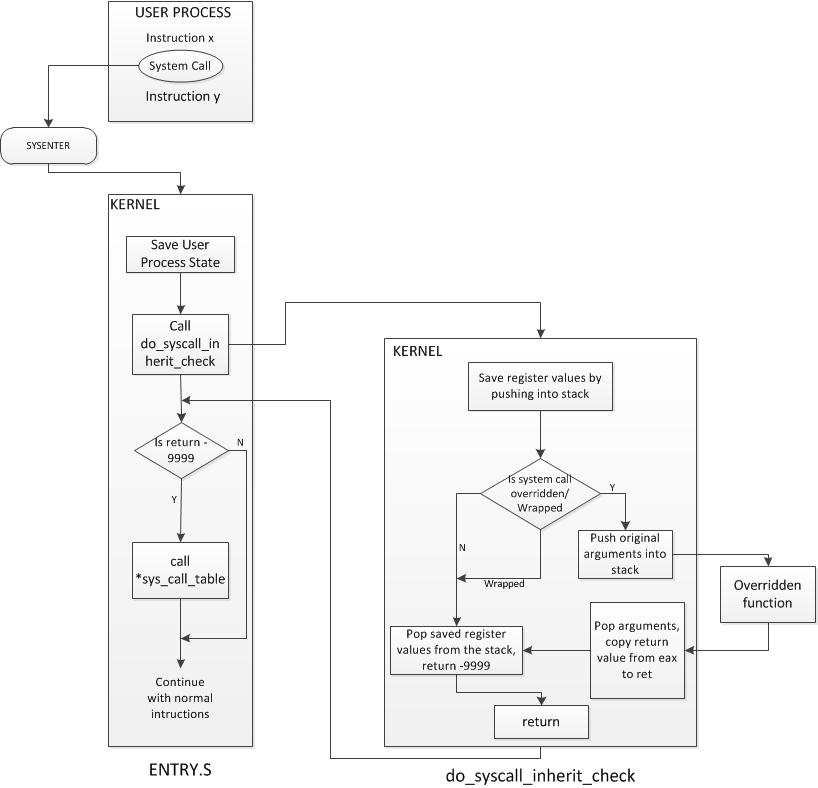
\includegraphics[width=5in]{control.jpg}
  \caption{Control Flow}
  \label{fig:ControlFlow}
\end{figure}


\subsection{Calling new system call handler}

In the existing system call handler, the arguments are pushed on to
the stack. The $\%eax$ register will have the system call number. In practice, $entry\_32.S$
calls the syscall table with syscall number in $\%eax$. Syscall table uses $\%eax$
as an index/offset for the table and then calls the respective memory
location in which the actual system call is present. System calls are
declared as $asmlinkage$ forcing the kernel to take the arguments from
the kernel stack.

In order to call our function implementation, we first send the control to our function
$do\_syscall\_inherit\_check$  from  $entry\_32.S$, where we check whether the private data field of $task\_struct$ is $NULL$ or not. But before calling we push $\%eax$ into stack to retain the value even after we call
our own function which tests if a system call is overridden, as we
need the $\%eax$ value if we find that the function is not overridden, to call the actual system call.
[Refer : ~\ref{fig:ControlFlow} on ~\pageref{fig:ControlFlow} ]

Inside $do\_syscall\_inherit\_check$, we first push all the register values(to
maintain their state in case the system call is not overridden) on to
the stack and then checks if the desired system call is overridden or not. 
If the system call is overridden, we call our function implementation by passing the
address of the function into $\%eax$ register and calling it.
Otherwise, we return $-9999$ into $\%eax$ register. But before returning,
we pop out all the values from the stack which we pushed during the intial phase in our function.

After we return from our call, we compare the return value in the $\%eax$ register with the top value in the stack
(original value $\%eax$ register which we pushed before our call to  $do\_syscall\_inherit\_check$
in $entry\_32.S$. If found that it is overridden, the call to syscall table is skipped, the $\%eax$ value that is
pushed earlier is popped into a register (it should not be popped into $\%eax$, we used $\%ebx$) and normal execution
is continued.  If the system call is not overridden, the earlier pushed  $\%eax$
value is popped into $\%eax$ and a call to syscall table is executed and
the instructions in $entry\_32.S$ are excuted as it would have for a normal system
call.

\subsection{Arguements Passing}

System calls are declared as $asmlinkage$ forcing the kernel to take the arguments from the kernel stack. We use this
same concept and declare the function implementation of overridden system call
as $asmlinkage$. For these overridden functions to work properly, we
prepare a stack frame as the kernel would do by pushing the arguments
in the right order. We push the original function arguments into the
stack by doing some arithmetic operations on the base pointer. [Refer : ~\ref{fig:kernelstack} on ~\pageref{fig:kernelstack} ]
We then call our function implementation of the overridden system call, this is done by moving the
address of the function implementation into $\%eax$ register and then making a call to it. 
After the function call, we get the return value of the system call function in $\%eax$ register,
 we copy it as the return value of our function i.e. $do\_syscall\_inherit\_check$, pop out all the values that we have pushed as
arguments to the overridden function, and finally return to $entry\_32.S$. So, now $\%eax$ register is populated with the
return value of the function $do\_syscall\_inherit\_check$, which in turn stores the return value of our function implementation of overridden system call.

\begin{figure}[hb2]
  \centering
  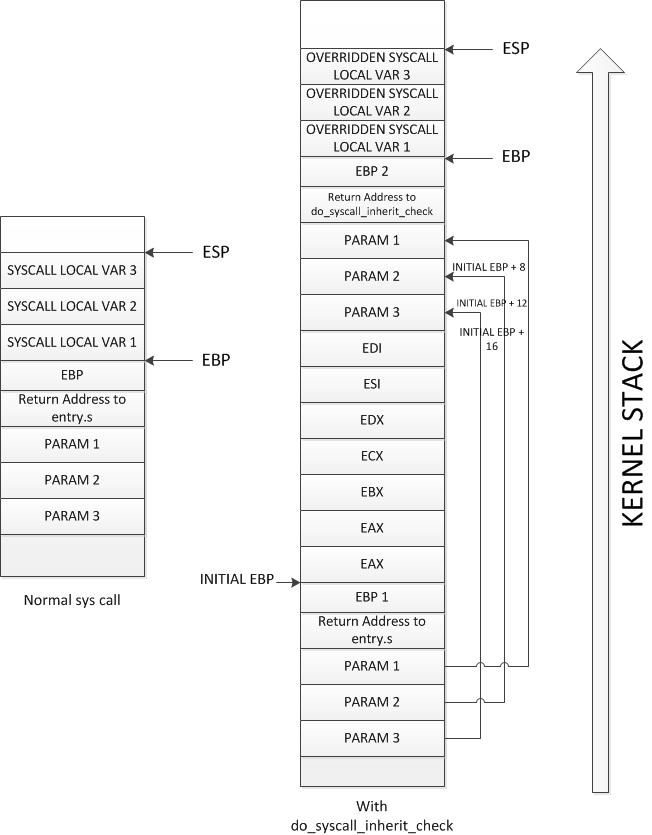
\includegraphics[width=5in]{kernel.jpg}
  \caption{Kernel stack}
   \label{fig:kernelstack}
\end{figure}

\section{Limitations and Advantages}

\begin{enumerate}[(a)]
\item
We are using ioctl as our method of communicating the vector name to kernel so that the $ioctl\_device$ module can find the $vector\_address$ corresponding to vector name and add it to the task structure. Along with adding to task structure we are also incrementing the reference count of module implementing the vector asked for by doing a $try\_module\_get()$ on that module.

To reduce the reference count we have to have some mechanism to know when the user process ends, which is not possible unless we monitor state of that process continuously. So instead, we created another IOCTL which the user process will explicitly call to notify the kernel to strip the vector address from the task structure of that process. In this call itself we reduce the reference count of the module, implementing the vector, by doing $module\_put()$ on that module. 

Now the drawback in this approach is that the user process has to explicitly do a $remove\ vector$ ioctl call so that reference counts are updated. So, if the user process, having new vector address in its task structure, is killed in between, while it is still working, will leave all modules in inconsistent state. (But this scenario will cause modules to be in inconsistent state, if we had used our own defined exec system call, other approach that we mentioned in proposal.)

Also this can't be called a drawback completely, it has a hidden advantage as well. It allows a user process to decide when it wants to use the overridden system calls and when original system calls. So, in a single process execution a process can call $IOCTL\_SET\_VECTOR$ to use one vector at one time say 'file\_ops\_vector' then call $IOCTL\_REMOVE$ to remove it and then again call $IOCTL\_SET\_VECTOR$ to use another vector say 'link\_vector' and then remove it as well and use third vector or use original system calls altogether. 

This way single process at multiple times can use multiple vectors or original system call depending on user requirements. Also, observe that this is an advantage of using ioctl over our own defined exec system call, which takes in only one vector at a time and will use that throughout its execution.


\item
Other limitation is that, since we have made a change in $entry\_32.S$ to change the flow of execution of system call interrupt to have a check whether the process is using any overridden vector or not, this makes our implementation architecture dependant. But again, this is not much of a drawback, because otherwise also, for normal execution all architectures have different way of handling the system call interrupt. That makes our implementation an adhesive part of normal system call interrupt, and a more reliable and stable way of implementation for future standard implementation of $system\_call\ inheritence$.

\item
One more drawback of having a new call $do\_check\_syscall\_vector$ in $entry\_32.S$, which checks for $void$* $syscall\_inherit\_data$ in task structure if it is empty or not, is that now a lot of CPU cycles are wasted in calling the function and doing the check. If we are inheriting only say 5 system calls, this check being made for all the system calls by any process, consumes lots of memory cycles and affects performance. We here leave a scope of improvement over this approach for future implementations and ideas.

\end{enumerate}

\section{Conclusion}

With the advent of Linux Kernel, the maintainers have made it more and more difficult to change the flow of system calls, may it be adding new system calls or system call overriding.  In order to keep people from doing potential harmful things $sys\_call\_table$ is no longer exported. In this paper we propose a mechanism to define new syscall vectors in which the existing system calls can be overridden or wrapped. We maintain the $asmlinkage$ functionality in the kernel by adding statements to maintain the kernel stack and by declaring the overriding/wrapping functions as $asmlinkage$. Since the users usually override/wrap few system calls only, we chose to add the syscall vector as a linked list and not as an array. This, not only helps us in adding other information necessary with the overridden/wrapped system calls but also saves precious kernel memory. We chose to implement an $ioctl$ instead changing the existing exec(and alike) or having a new version of exec, for maitaining kernel portability. We do this to provide an user the ability to change/remove syscall vectors at runtime. Also, we have implemented the inheritance of this new syscall vector that we have added by making changes to the process $task\ structure$; by adding a $void$ * field at the end of the structure thus making sure that we don't disturb the existing kernel code. We have successfully tested scenarios which we think are apt and these have been mentioned in appendix A.  


\section{References}

\begin{enumerate}[(a)]
\item
\url{http://lxr.fsl.cs.sunysb.edu/linux/source/}

\item
\url{http://www.informit.com/articles/article.aspx?p=370047}

\item
\url{http://www.ibiblio.org/gferg/ldp/GCC-Inline-Assembly-HOWTO.html#s2}

\item
\url{http://www.cs.lmu.edu/~ray/notes/x86assembly/}

\item
\url{http://articles.manugarg.com/systemcallinlinux2_6.html}

\item
\url{http://www.win.tue.nl/~aeb/linux/lk/lk-4.html}

\item
\url{http://linux.die.net/lkmpg/x978.html}

\item
\url{http://kernelnewbies.org/FAQ/asmlinkage}

\item
\url{http://kernelnewbies.org/FAQ/asmlinkage}

\item
\url{http://stackoverflow.com/questions/10060168/is-asmlinkage-required-for-a-c-function-to-be-called-from-assembly}

\item
\url{http://www.win.tue.nl/~aeb/linux/lk/lk-4.html}

\item
\url{http://www.csee.umbc.edu/~chang/cs313.s02/stack.shtml}

\end{enumerate}

\newpage

\appendix

\section*{Appendix}

\section{ Test Cases}

We plan to have the demo with two syscall vectors that we are adding: 

\noindent
 \textbf{1. file\_ops\_vector}

    a. open(wrapped) : prints the arguments passed and returns a value indicating that open is only wrapped  

    b. fchown(overridden): prints the arguments

    c: read: (overridden): puts data(random\_text) in the data buffer passed by the user. 

\medskip
\noindent
\textbf{2. link\_vector}

    a. link(overridden): prints old pathname and new pathname

    b. unlink(wrapped): prints some statements and returns indicating that this call was just overridden

\medskip
\noindent
\textbf{Test1:}

User Program has the new system call vector: $file\_ops\_vector$. 

User Program calls:

1. open with $test1\_file$, $O\_CREAT$ and 777 as arguments. 

2. read with as arguments 100(random file decriptor), user buffer, 200(read size)

3. fchown with 11,22,33(all random) as arguments 

\noindent
\textbf{Expected Output: }

1. Since open is just wrapped, the arguments are printed on the screen from the wrapped function and original system call is called thus creating the file, $test1\_file$

2. the overridden read function puts text: $random text$ into the user buffer. 

3. Prints the arguments. 

\medskip
\noindent
\textbf{Test2:} 

User program has a new system call vector: $link\_vector$. 

User Program calls:

1. link with $link\_old$ and $link\_new$ as arguments

2. unlink with $test1\_file$ as arguments. 

\noindent
\textbf{Expected Output: }

Since link is just overridden, the arguments are jsut printed.

Since Unlink is wrapped, some statements are printed inside the wrapped function and the wrapped function returns with a value indicating that the function is just wrapped. Thus, original system call unlink is called with $test1\_file$ as argument, thus removing that file.

\medskip
\noindent
\textbf{Test3:} 

User Program has the new system call vector: $file\_ops\_vector$ 

We have used fork to create a child process. 

Parent Process calls open with test3\_parent, O\_CREAT and 777 as arguments. 

Child Process calls fchown with 11,22,33(all random) as arguments 

\noindent
\textbf{Expected Output: }

Since open is just wrapped, the arguments are printed on the screen from the wrapped function and original system call is called thus creating the file, test3\_parent

This test proves to be important as we are showing the functionality of system call inheritance by using fork. This test proves that even the child process' task structure is updated with the parents task struct. Thus, overridden fchown in the child is this called and just prints the arguments. 

\medskip
\noindent
\textbf{Test4:} 

User Program has the new system call vector: link\_vector. 

We have used fork to create a child process. 

Parent Process calls link with test4\_oldpath and test4\_newpath as arguments

Child Process calls unlink with test3\_parent (which was created in test3) as argument.

After child process returns, parent process sleeps for sometime. 

Then the parent process removes link\_vector from its task structure. 

\noindent
\textbf{Expected Output:} While the parent process is sleeping, we see that link\_vector is still associated with it. If we try to remove the vector module, if the reference counts had been handled properly, we should not be able to remove the link vector module. We check this while the process is sleep. After is returns from sleep, the process itself will remove the vector from its task struct. Then after the program exits, you can remove the link vector module successfully. 


\medskip
\noindent
\textbf{Test5: }

Initially the user Program has the new system call vector: file\_ops\_vector. Open system call is called with test5\_file, O\_CREAT, 777 as arguments. Then user program at run time removes this vector, sleeps for sometime and adds the link\_vector Now unlink system call is made with test5\_file as arguments. Then user program removes link\_vector and then sleeps for sometime and then calls open with test5\_new\_file, O\_CREAT, 777 as arguments. 

\noindent
\textbf{Expected Output: }

test5\_file is created because the wrapped open system from file\_ops\_vector call is called. Then the process removes this vector and adds link\_vector to the We added sleep in between so that we can ssh and show that the file is being created while the process sleeps.Then, unlink from the link\_vector is called. Then the file test5\_file will be removed since the unlink system call is just wrapped in link\_vector. We have put a sleep again to confirm this by doing an ls and dmesg. Then link\_vector is removed from the process' task structure. Then because of the open system call creates the test5\_new\_file as expected and through the dmesg command we can confirm that there are no overriding system call vectors. 

\section{Code Changes}

\begin{enumerate}[(a)]
\item
Added a new $void$ * field $syscall\_inherit\_data$ in the struct $task\_struct$ in $/usr/src/hw3-cse506g12/include/linux/sched.h$

\item
Added an exteren declaration of $do\_syscall\_inherit\_check$ function in $/usr/src/hw3-cse506g12/arch/x86/include/asm/signal.h$ 

\item
Modified $/usr/src/hw3-cse506g12/arch/x86/kernel/entry\_32.S$ 

\item
Definition of $do\_syscall\_inherit\_check$ function defined in $/usr/src/hw3-cse506g12/syscall\_inherit/syscall\_inherit.c$.

\item
All the four \textbf{LKM}'s (Loadble Kernel Modules) are present in $/usr/src/hw3-cse506g12/hw3/os\_proj$. 

\end{enumerate}

\section{How To Run}

\begin{enumerate}[(a)]
\item
git clone ssh://user@scm.cs.stonybrook.edu:130/scm/cse506git-s12/hw3-cse506g12
\item
cd hw3-cse506g12
\item
cp kernel.config .config
\item
make
\item
make modules\_install 
\item
make install
\item
reboot
\item
cd /usr/src/hw3-cse506g12/hw3/os\_proj
\item
./clean.sh
\item
./make.sh
\item
cd test\_demos
\item
./test1 file\_ops\_vector
\item
./test2 link\_vector
\item
./test3 file\_ops\_vector
\item
./test4 link\_vector
\item
./test5
\end{enumerate}

\end{document} 